\documentclass[conference]{IEEEtran}
\IEEEoverridecommandlockouts
% The preceding line is only needed to identify funding in the first footnote. If that is unneeded, please comment it out.
\usepackage{cite}
\usepackage{amsmath,amssymb,amsfonts}
\usepackage{algorithmic}
\usepackage{graphicx}
\usepackage{textcomp}
\usepackage{xcolor}
\usepackage{multicol}
\usepackage{amsmath}
\def\BibTeX{{\rm B\kern-.05em{\sc i\kern-.025em b}\kern-.08em
    T\kern-.1667em\lower.7ex\hbox{E}\kern-.125emX}}
\begin{document}

\title{Prediction of the cryptocurrency market\\ using Azure ML\\
%\thanks{Mr PEJMAN Rasti -- Teacher of the DataMining Course}
}

\author{\IEEEauthorblockN{BARBAULT Cyprien}
\IEEEauthorblockA{\textit{Big DATA Student} \\
\textit{ESAIP -- Engineering School}\\
Angers, France \\
cbarbault.ing2022@esaip.org}
\and
\IEEEauthorblockN{GIROU Romain}
\IEEEauthorblockA{\textit{Big DATA Student} \\
\textit{ESAIP -- Engineering School}\\
Angers, France \\
rgirou.ing2022@esaip.org}
\and
\IEEEauthorblockN{MOTHELAY Xavier}
\IEEEauthorblockA{\textit{Big DATA Student} \\
\textit{ESAIP -- Engineering School}\\
Angers, France \\
xmothelay.ing2022@esaip.org}
}

\maketitle

\begin{abstract}
This document is a sum up of our project mixing machine learning and cryptocurrencies. We describe the current situation of the cryptocurrency and how we decided to build our algorithm on Azure Machine Learning Studio.
\end{abstract}

\begin{IEEEkeywords}
Bitcoin, Cryptocurrency, Machine Learning, Market, Microsoft Azure
\end{IEEEkeywords}

\section{Introduction}

For the course of Data Minning, we were given the opportunity to choose a subject to work on to apply one of the different type of AI seen in classe (Regression, Classification, NLP, Computer vision, \dots). We opted for the application of regression through the prediction of the crypto-currency market. 

\section{Why using the Machine Learning in the crypto-currency market ?}

\subsection{The world of cryptocurrencies}

In 2009, the Bitcoin, future leader of the market of the cryptocurrencies was created. This money of a new type was based on the original concept of \textbf{David Chaum}. As a reminder, this is the definition of a crypto currency by the Cambridge Dictionary :\\
\begin{quote}
A digital currency produced by a public network, rather than any government, that uses cryptography to make sure payments are sent and received safely.\cite{b1}\\
\end{quote}

Cryptocurrencies can be ``mined''\footnote{With GPU or ASICS, not in real mines} and offered as a reward to the ``miners''. Those miners are then able to sell the fruit of their work, as a result, the crypto (short for cryptocurrency) acts like a Forex market. As miners gather more and more crypto, the quantity of currency on the market is increasing, and thus the complexity of the mining increase to avoid overflooding the market.\\

With the use of the \textbf{blockchain technology}, cryptocurrencies (and the Bitcoin in particular) are offering security and anonymity to its buyers and seller on every transaction.\\


\subsection{Cryptocurrencies market's problem }

Because of their lack of centralisation, cryptos-markets are highly volatiles. The Bitcoin for example have already gained more than 3000\$ in a day and lost more than 50\% of its value in the same duration\cite{b2}. Crypto investor have to be really precautious with such a market, and in order to maximise their gain, the solution could be the machine learning. ML (short for Machine Learning) is the use of a big amount of data to train an algorithm in a specific task with the help of statistics. 

\subsection{Machine learning in the tradding world}

The bitcoin market, it's more than 350k transactions a day ! With such a number of transactions, we have a ton of data to analyse\dots{}~And people understood that, more and more people are trying to predict Bitcoin price a month, a week, a day of even a few seconds aheads. If you can predict how the currency will behave, you know when to buy and when to retire.\\

We now we won't get rich with a simple regression model on Azure (or everybody would do it), but we wanted to put a foot in this field, and understand both how machine learning and markets works so we decided to see how accuratly we could predict the price of various cryptos just one minute ahead

\subsection{The Dataset}

We picked a dataset based on \textbf{Gemini}'s data over the BTC/USD, ETH/USD, ZEC/USD and LTC/USD every minutes of the 2019 year.\footnote{Bitcoin to US dollar, Etherum to US dollar, Zcash to US dollar and Litecoin to US dollar}. This Dataset is made out of 1.751.122 entries ($\dfrac{1}{4}$ of each coin) and is based on 8 columns : 
\begin{multicols}{2}
\begin{itemize}
\item UNIX Timestamp
\item Symbol
\item Open
\item High
\item Low
\item Close
\item Volume
\item Date
\end{itemize}
\end{multicols}

\subsubsection*{UNIX Timestamp and Date} The UNIX Timestamp is the elapsed time (in seconde) since the January, $1^{\textrm{st}}$ 1970 while the date is\dots~ the date and hour of the timeframe\\

\subsubsection*{Symbol} The symbol of the crypto (BTC,ETH,LTC,ZEC)\\

\subsubsection*{Open/Close} Respectively the price of the currency at opening and closing of the market (at the beginning and the end of each minute)\\

\subsubsection*{High/Low} Respectively the price of the currency at its highest and lowest during the timeframe (each minute)\\

\subsubsection*{Volume} Number of tokens exchanged during the timeframe


\subsection{Dataset preparation}

First thing to know is that we didn't really had a dataset with the four currencies. In fact, what we really had was four datasets, each about a different crypto. So we had to concatenate the differents datasets into on big dataset. Thankfully, Azure ML is offering this kind of option in the dataset section, you can pick differents \texttt{.csv} files with the same header and make one big dataset of it.\\

The second action we took to prepare our dataset was the selection of the columns we wanted. For example, the UNIX Timestamp was worthless. We also needed to get rid of the Date column because it had differents format between the differents crypto we picked, so to avoid conflicts, we decided to remove it entirely.\\

For security, we also cleant the data by removing line where some fields were missing. But as the source of the datasets was \textbf{Gemini}, we didn't expected to loose a lot of it.\\

Then we had to normalize the Data. We picked the \textbf{MinMax} transformation method to set the value of \texttt{Open,Low,Close} and \texttt{Volume}\footnote{These columns will be the feature for ou ML algorithm} in a range of 0 to 1 to speed up the training time.

Finnaly, we splitted the data between the training set (70\% of the dataset) and the test set (the 30\% left). This way, we could see if the trained model is accurate or not.

\subsection{The choice of the model}

When it comes to the choice of a model for our machine learning algorithm, we initialy planned to go for the \textbf{Linear Regression Model}. But in order to be sure it was the right model for the task, we finnaly decided to compare four differents models:
\begin{itemize}
\item Linear Regression
\item Poisson Regression
\item Machine Learning Regression
\item Random Forest Regression
\end{itemize}

Note that we will concentrate on the MAE (Mean Absolute Error) only for this comparison.\\
\begin{table}[!h]
\begin{center}
\begin{tabular}{|c|c|}
\hline
\textbf{Model} & \textbf{MAE}\\
\hline
Random Forest Regression & 0.500912 \\
Linear Regression & 1.13083 \\
Poisson Regression & 88.58514\\
Machine Learning Regression  & 3639.995401 \\
\hline
\end{tabular}
\end{center}
\caption{Score of the differents models}
\end{table}

We had a clear winner: the \textbf{Random Forest Regression Model} 

\subsection{Results}

\begin{figure}[h!]
\begin{center}
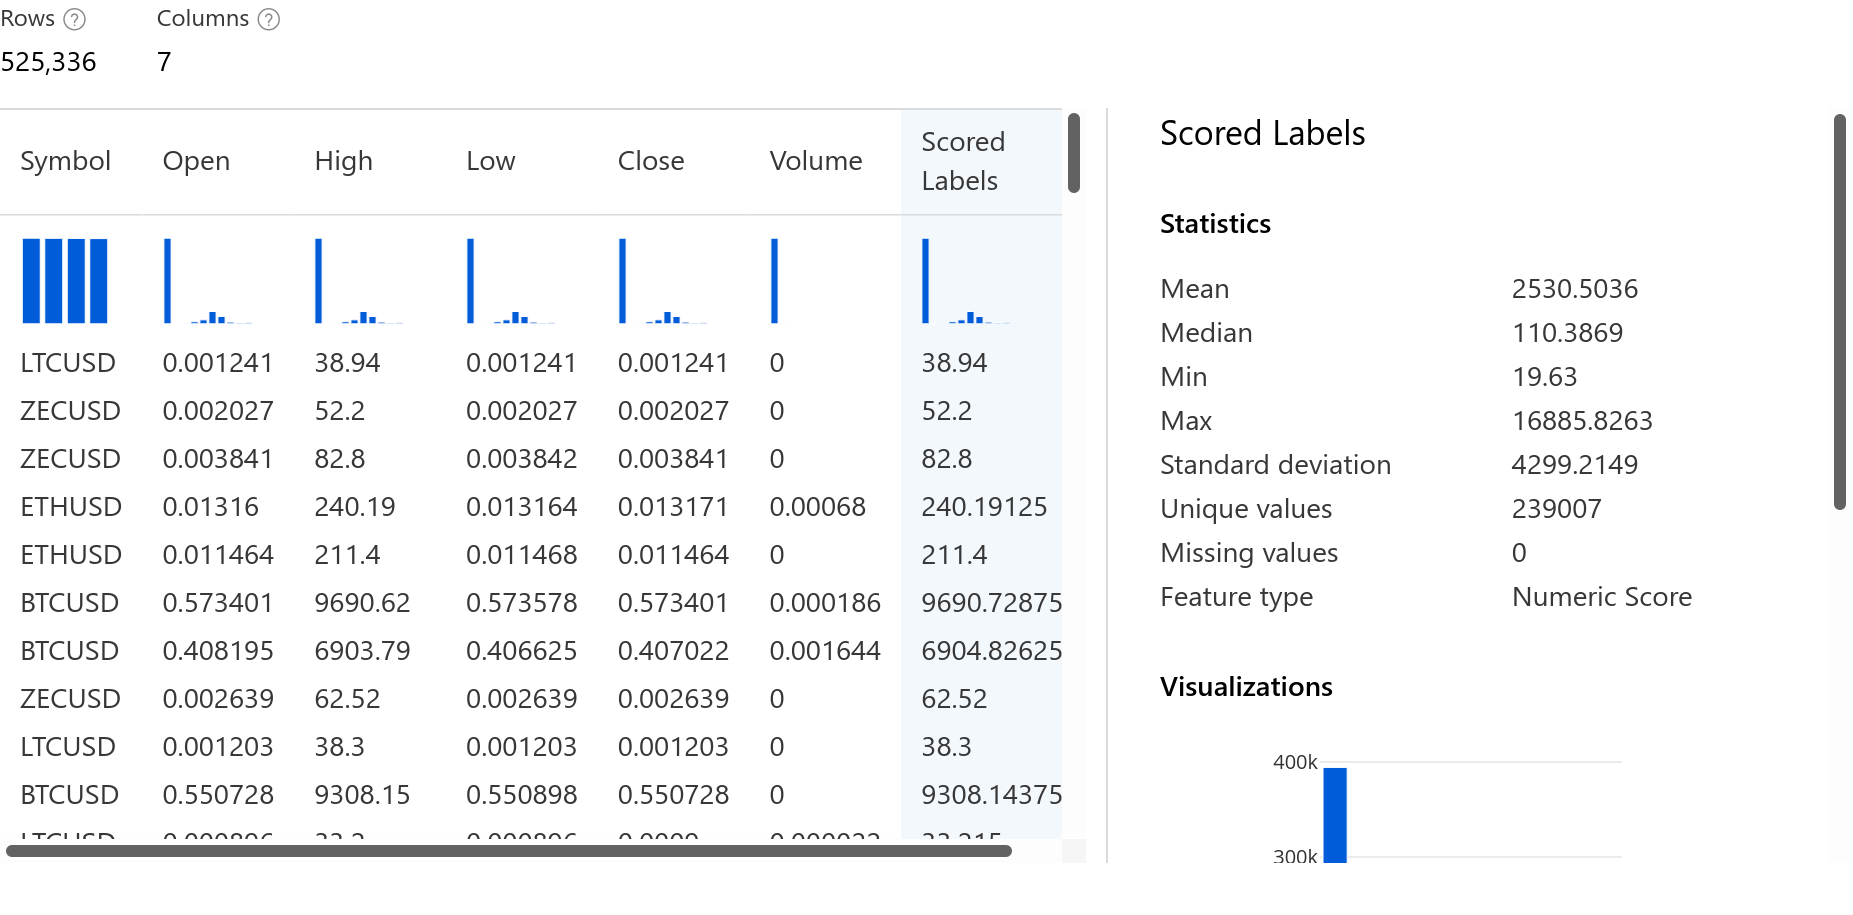
\includegraphics[scale=0.15]{rd_forest_reg.png}
\end{center}
\label{fig:results}
\caption{Results obtained with the Random Forest Regression Algorithm}
\end{figure}

\subsubsection*{Analysis} As we can see on the figure \ref{fig:results}, the \textbf{High} column in the column we wanted to predict and the \textbf{Scored Labels} is the predicted result. The results are really close !\\

If you imagine linking an trading algorithm to this model, then you can predict the highest price of a time frame. This way, if your buying price is lower than the highest price, your trading bot could sell automatically your crypto and gain a significant margin !

\section{Conclusion}

Crypto-currencies may be the currency of the future, and we must prepare ourself for a world where the market is full of micro-transaction at really high frequency. A world where transactions could be totaly anonymous and untraceable. In this world, BOT and AI would rule the market and billions of dollars would be traded each seconds. In this world there would be no place for errors\dots~ To avoid dramatics lost for some companies, AI have to be trained to predict with accuracy the fluctuations of the market. \\
Our goal was to predict with precision the price of the highest value of the market at every minute. Even though our algorithm seems to be really good in this cas, this prediction is on the really short term, and in the real world, it may be more useful to predict the variation at a higher scale (on a week or a month). An improvement we could make to our project is to change the dataset for a dataset based on the evolution of the market on a daily basis or even try to predict some days in advance instead of the current minute. An other approach would be to use the sentiment analysis, for example on Twitter, to measure the confidence, this could be a good idea for a future projet.


\begin{thebibliography}{00}

\bibitem{b1} Definition of a Cryptocurrency, Cambridge Dictionary, https://dictionary.cambridge.org/us/dictionary/english/cryptocurrency

\bibitem{b2} Charles Bovaird, Bitcoin Lost Roughly 50\% Of Its Value In A Day, Mar 12 2020,  https://www.forbes.com/sites/cbovaird/2020/03/12/bitcoin-lost-roughly-50-of-its-value-in-a-day/



\end{thebibliography}
\vspace{12pt}
\color{red}
\end{document}